\chapter{Mesh Renumbering}\label{chapter:renumbering}

This program aims to be able to process unstructured meshes, to be more general and to be able to
perform computations on already available meshes. The program also aims to use the Hilbert curve, a
\acrlong{acr:SFC}, to preserve locality and reduce the size of inter-\acrshort{acr:GPU} boundaries.
The curve is described in Section~\ref{section:load_balancing:hilbert_curve}. These two objectives
are at odds, as the overwhelming majority of meshes that were created for other purposes will not be
numbered according to the Hilbert curve. Also, the Hilbert curve is only defined for square domains
with \(n\) axis-aligned quadrilateral elements in the \(x\) and \(y\) directions, where \(n\) is a
power of two. Therefore, most off-the-shelf will not inherit the good locality and small boundaries
between mesh blocks that we put a lot of effort to achieve in Chapter~\ref{chapter:load_balancing}.
Not only that, but there is even a performance penalty when using a single \acrshort{acr:GPU} if
elements that are close in the ordering are not geometrically close, as memory access patterns are
worsened. An extreme example is the original mesh used for
Section~\ref{section:results:complex_meshes}. Figure~\ref{fig:mesh_unsorted} shows the ordering of
the elements and how the mesh is split into mesh blocks if partitioned into \(16\) blocks as-is. 

\begin{figure}[H]
	\centering
	\subfloat[Ordering]
	{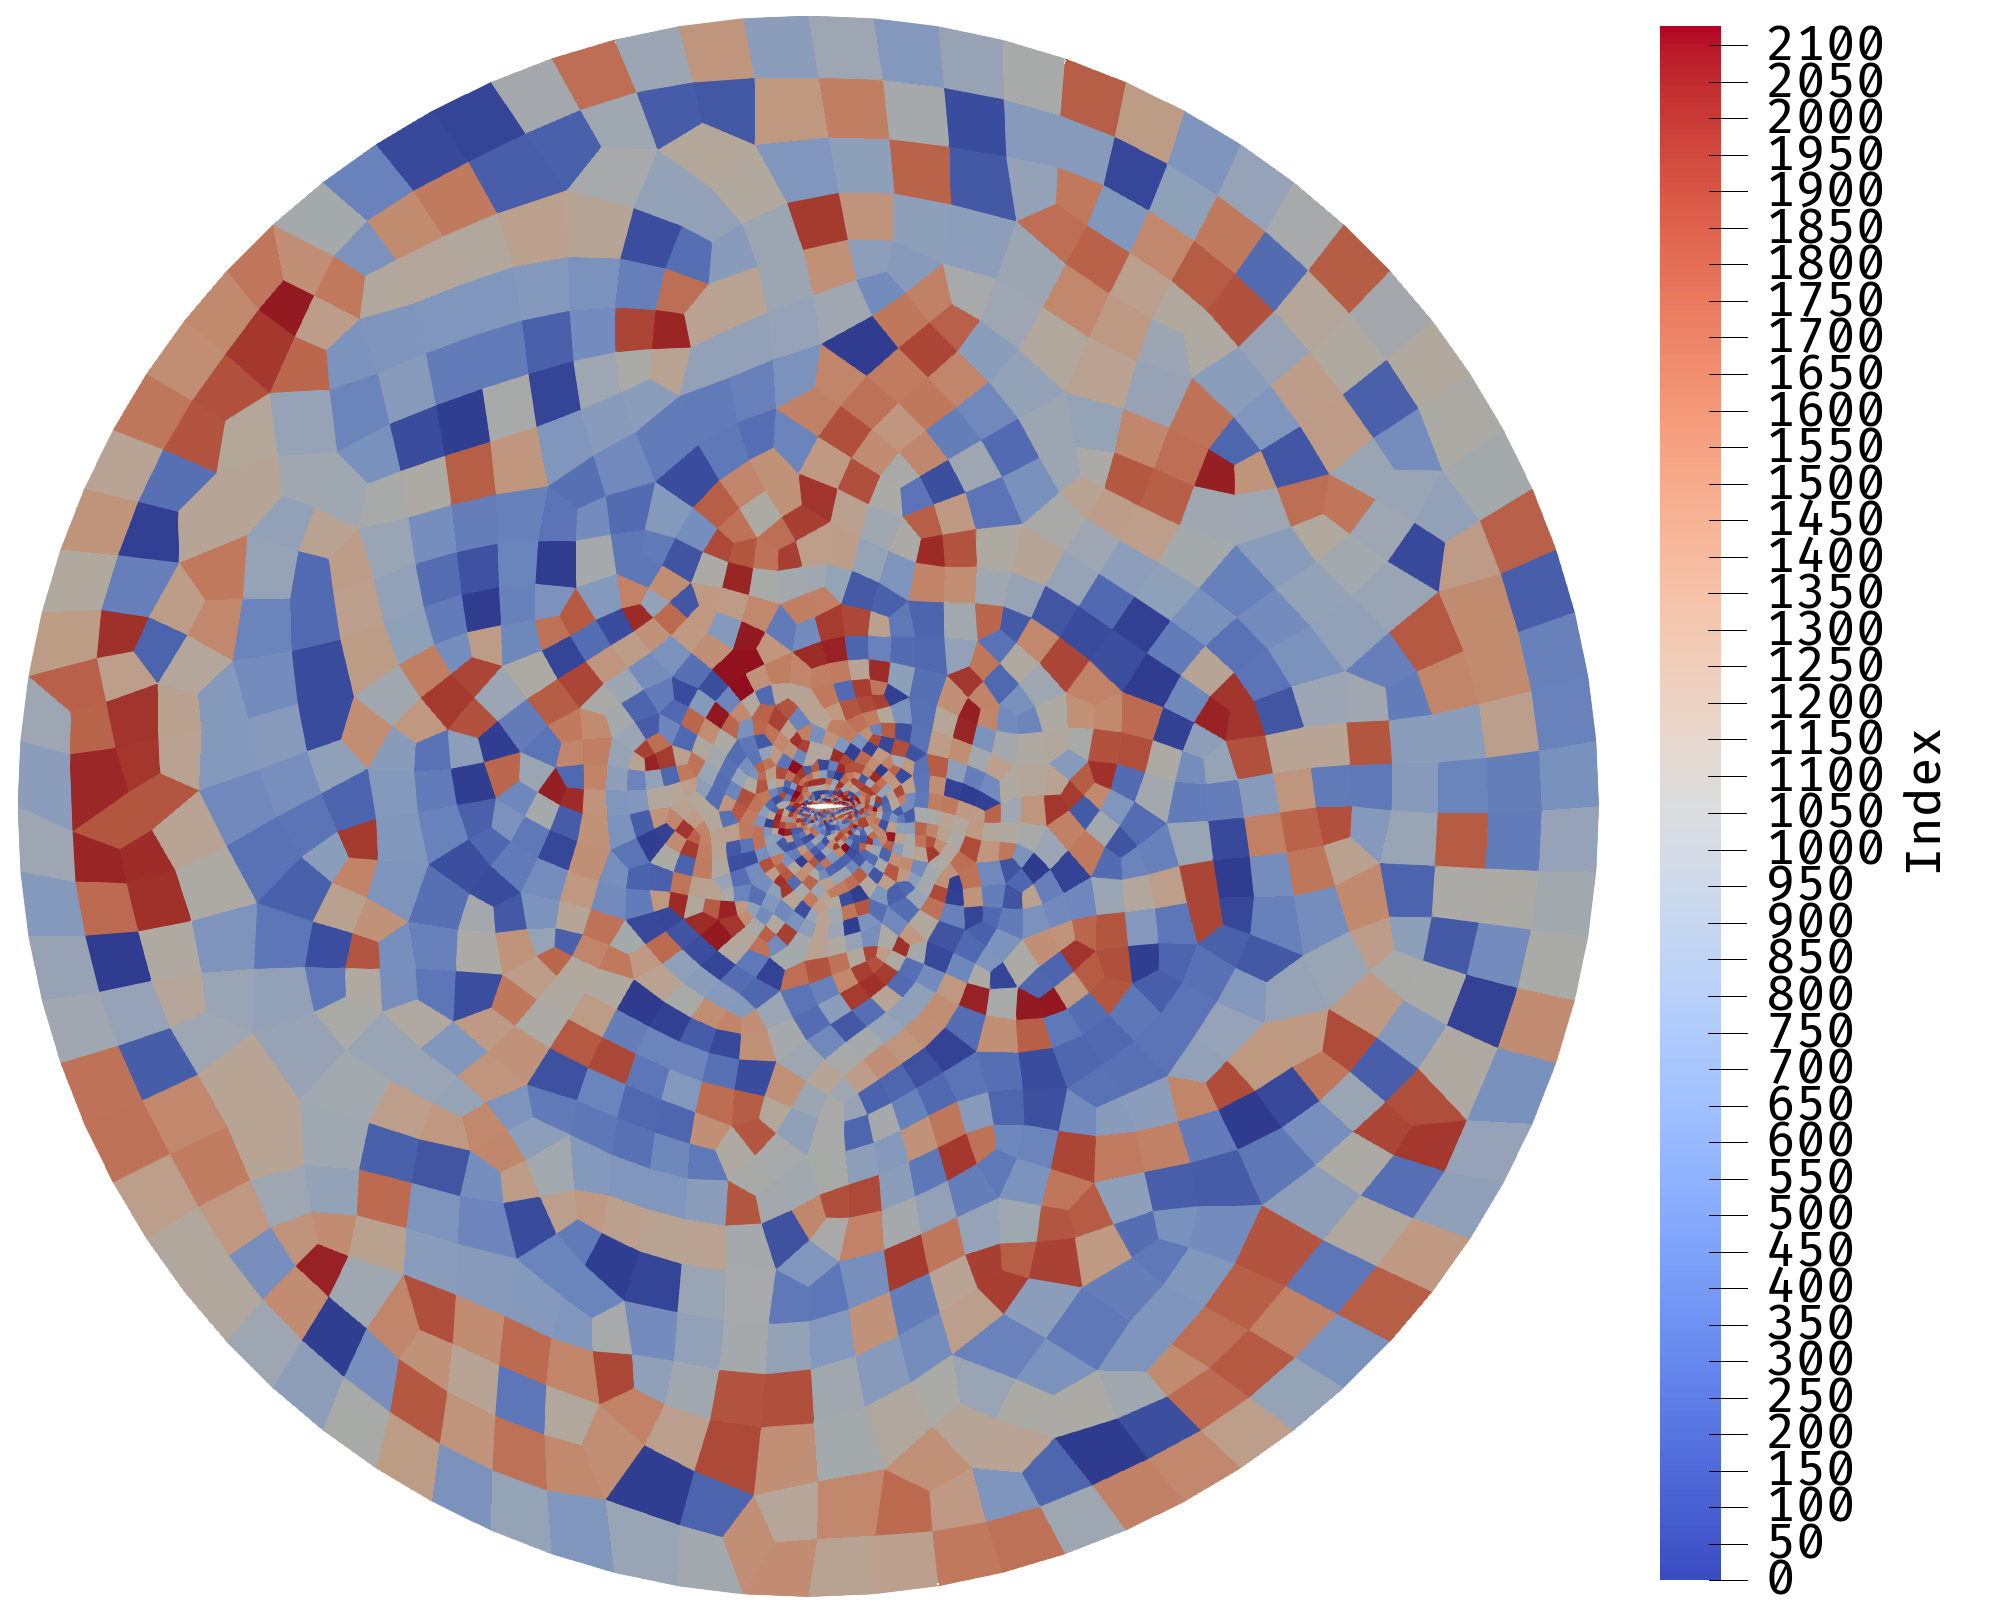
\includegraphics[width=0.45\textwidth]{Chapter_renumbering/media/ordering_unsorted}\label{fig:ordering_unsorted}}
	\subfloat[Rank]
	{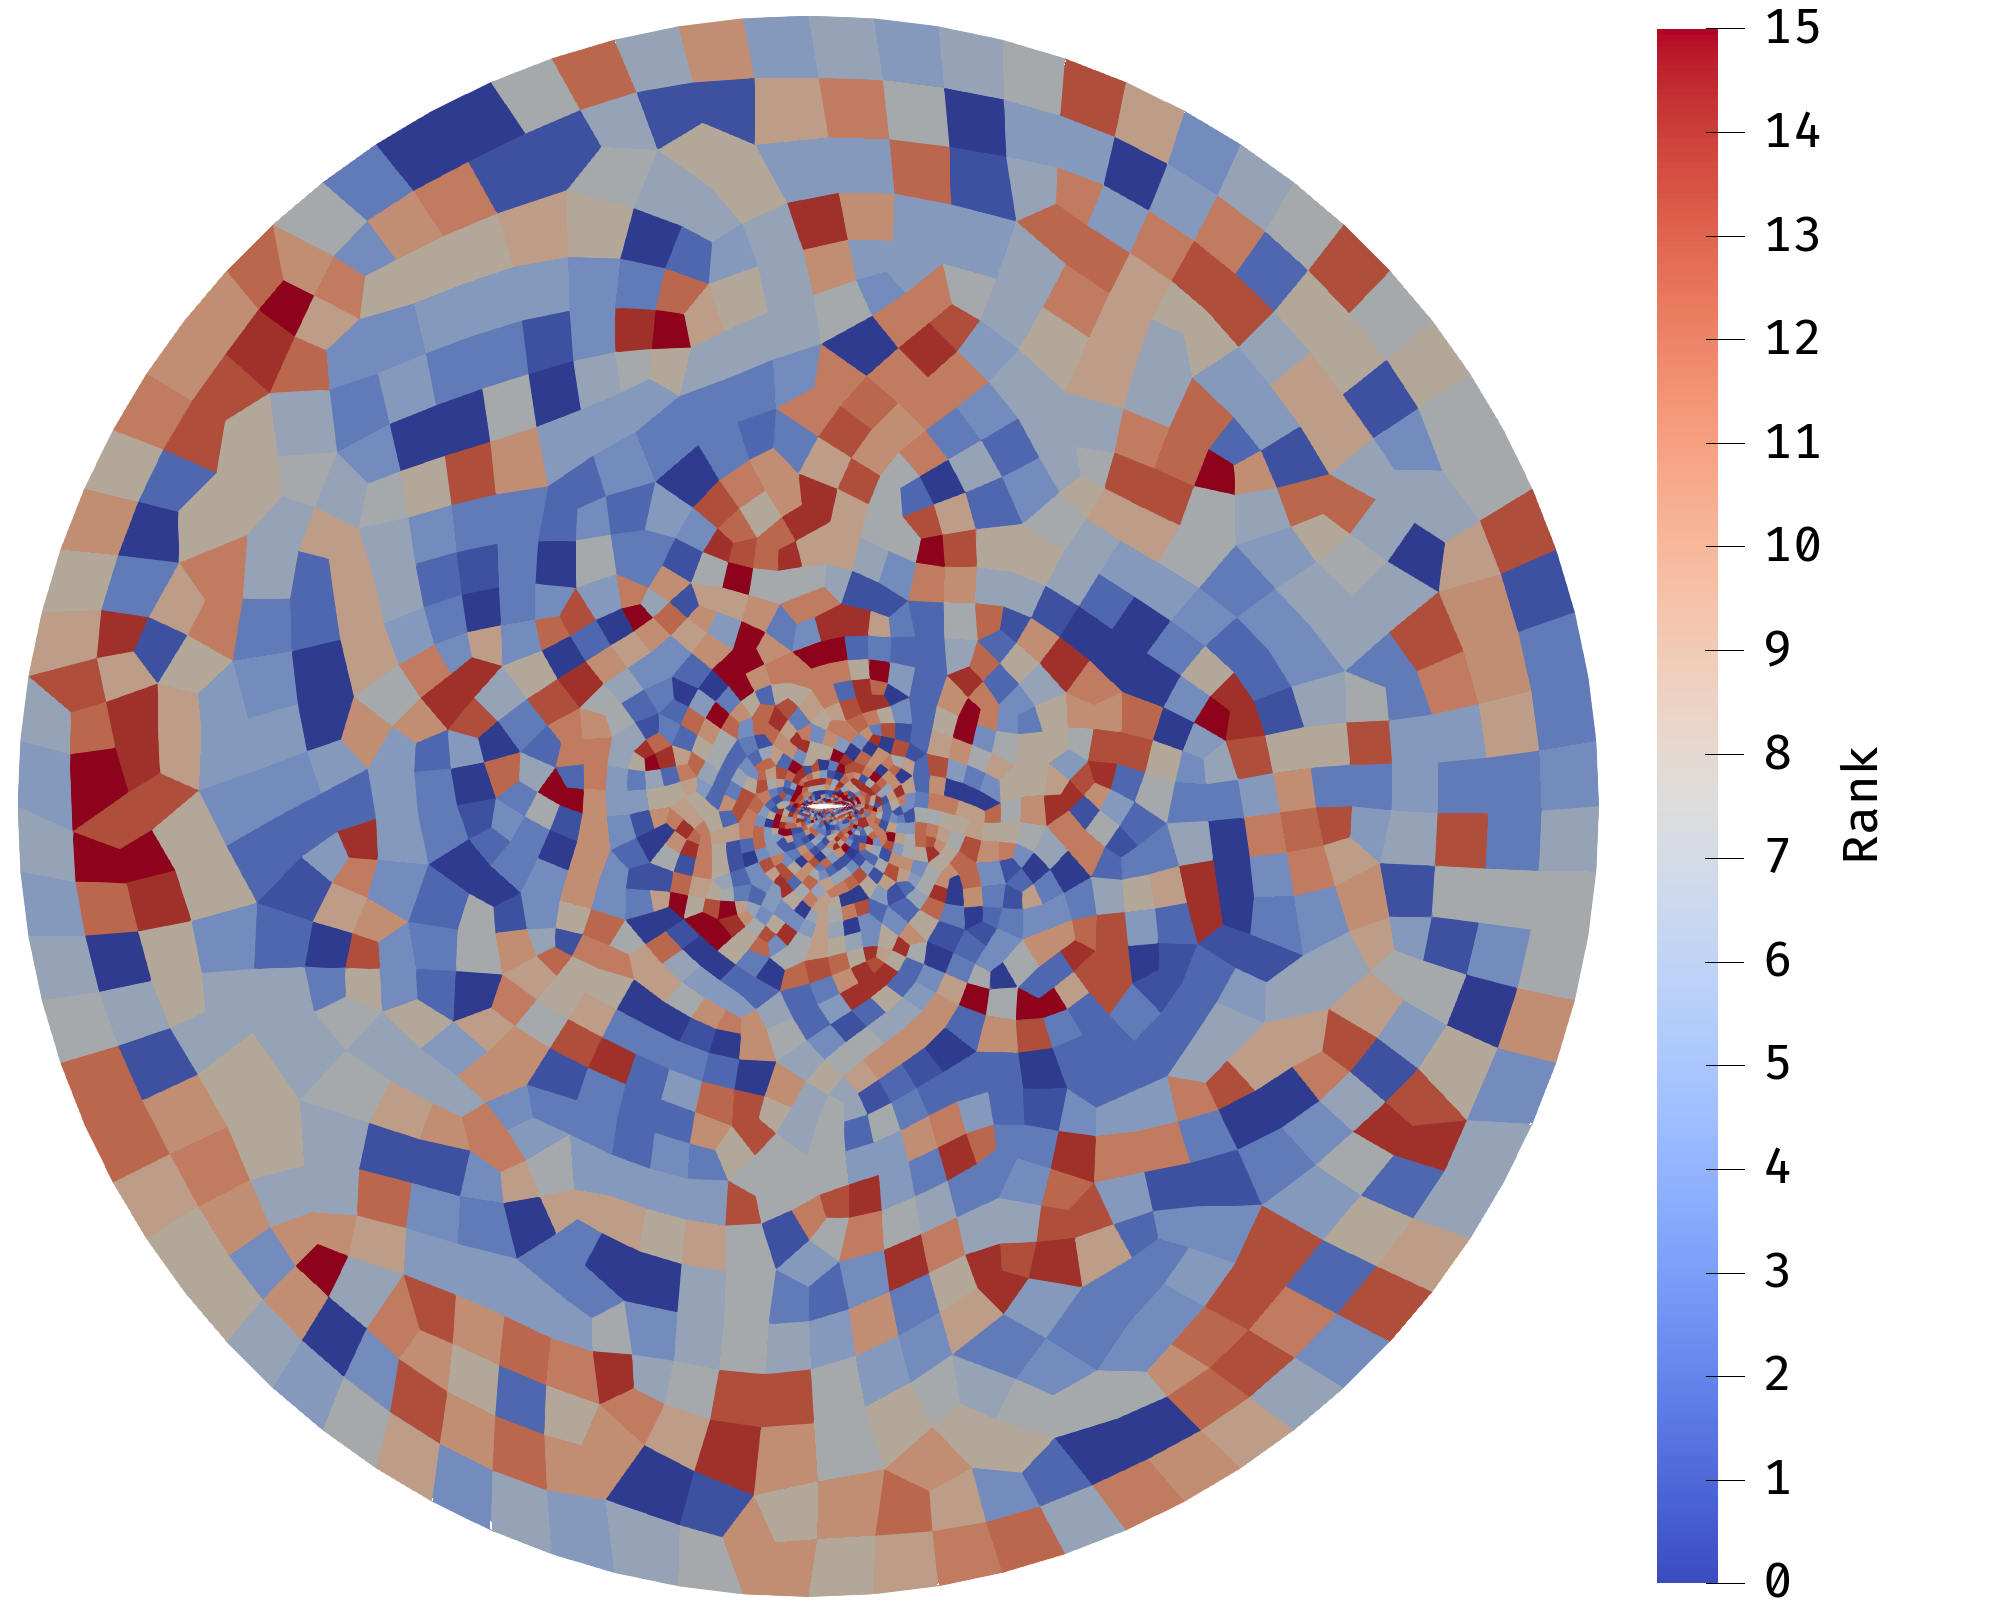
\includegraphics[width=0.45\textwidth]{Chapter_renumbering/media/rank_unsorted}\label{fig:rank_unsorted}}
	\caption{Unsorted mesh: The mesh is partitioned into \(16\) mesh blocks. (a) Ordering of the elements within the mesh (b) Mesh blocks once partitioned}\label{fig:mesh_unsorted}
\end{figure}

As we see, the resulting mesh blocks are scattered around the mesh, leading to unnecessarily large
boundaries between blocks. In order to get good performance, we will need to renumber the mesh. 

Since this mesh is circular, and the discontinuity representing the fuselage is in the middle, a
simple sorting algorithm could be to represent the elements in polar coordinates, and sort them
according to their angle around the center \(\theta \). Doing this, we get the ordering and
partitioning shown in Figure~\ref{fig:mesh_circular}.

\begin{figure}[H]
	\centering
	\subfloat[Ordering]
	{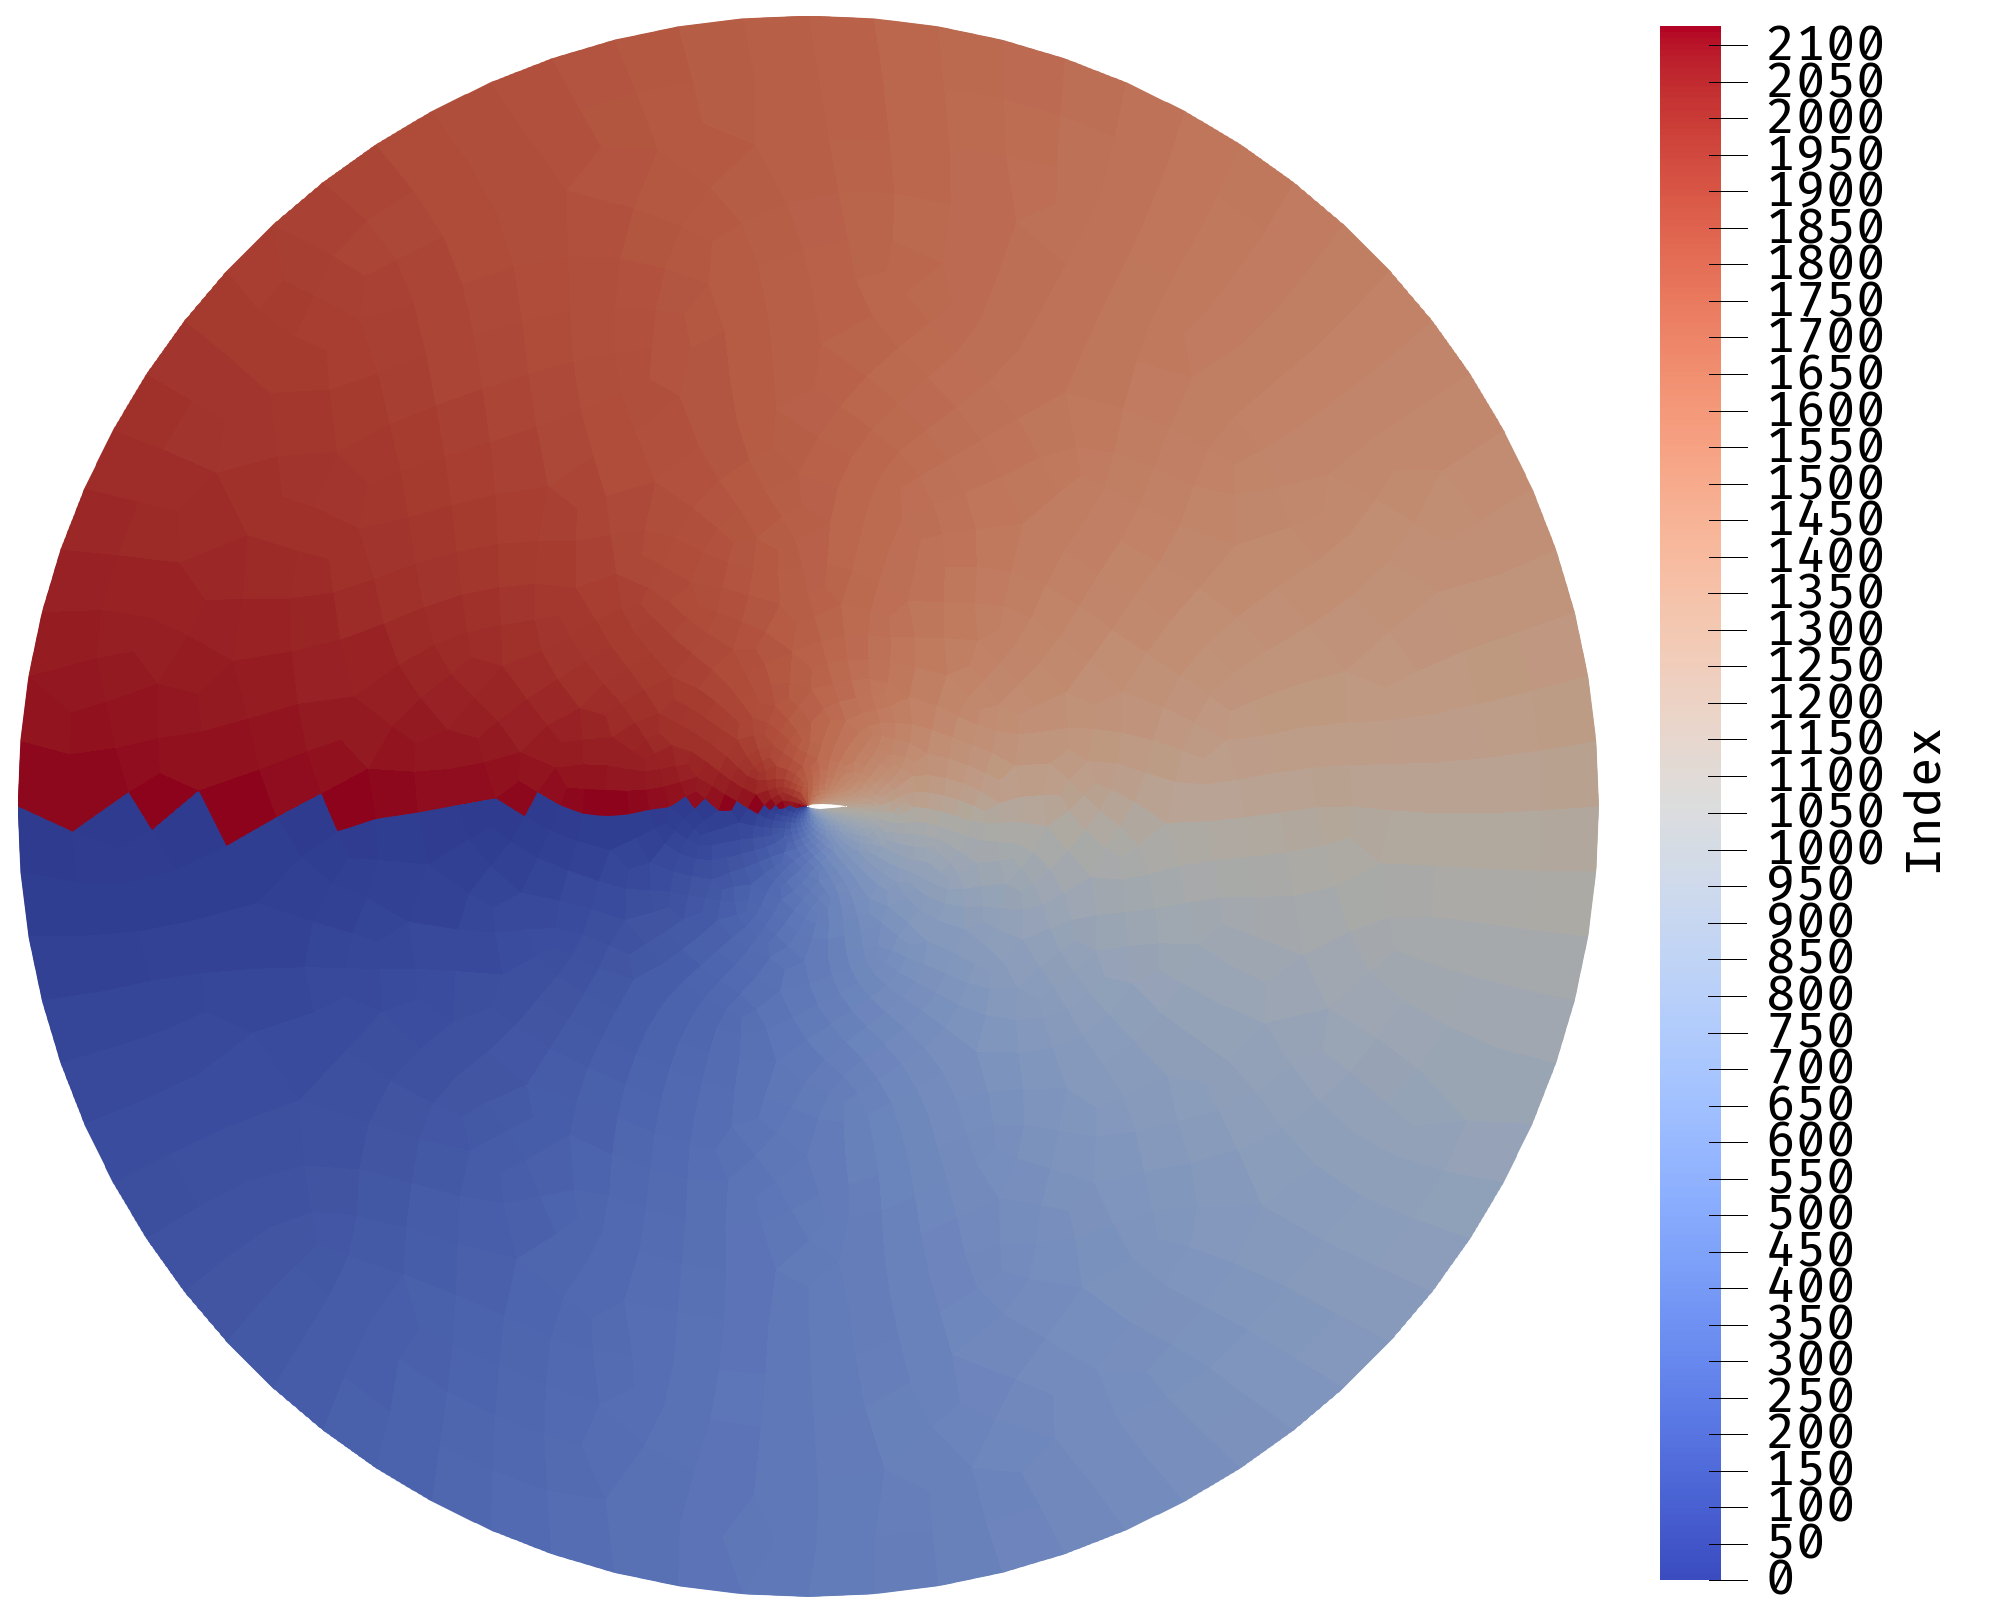
\includegraphics[width=0.45\textwidth]{Chapter_renumbering/media/ordering_circular}\label{fig:ordering_circular}}
	\subfloat[Rank]
	{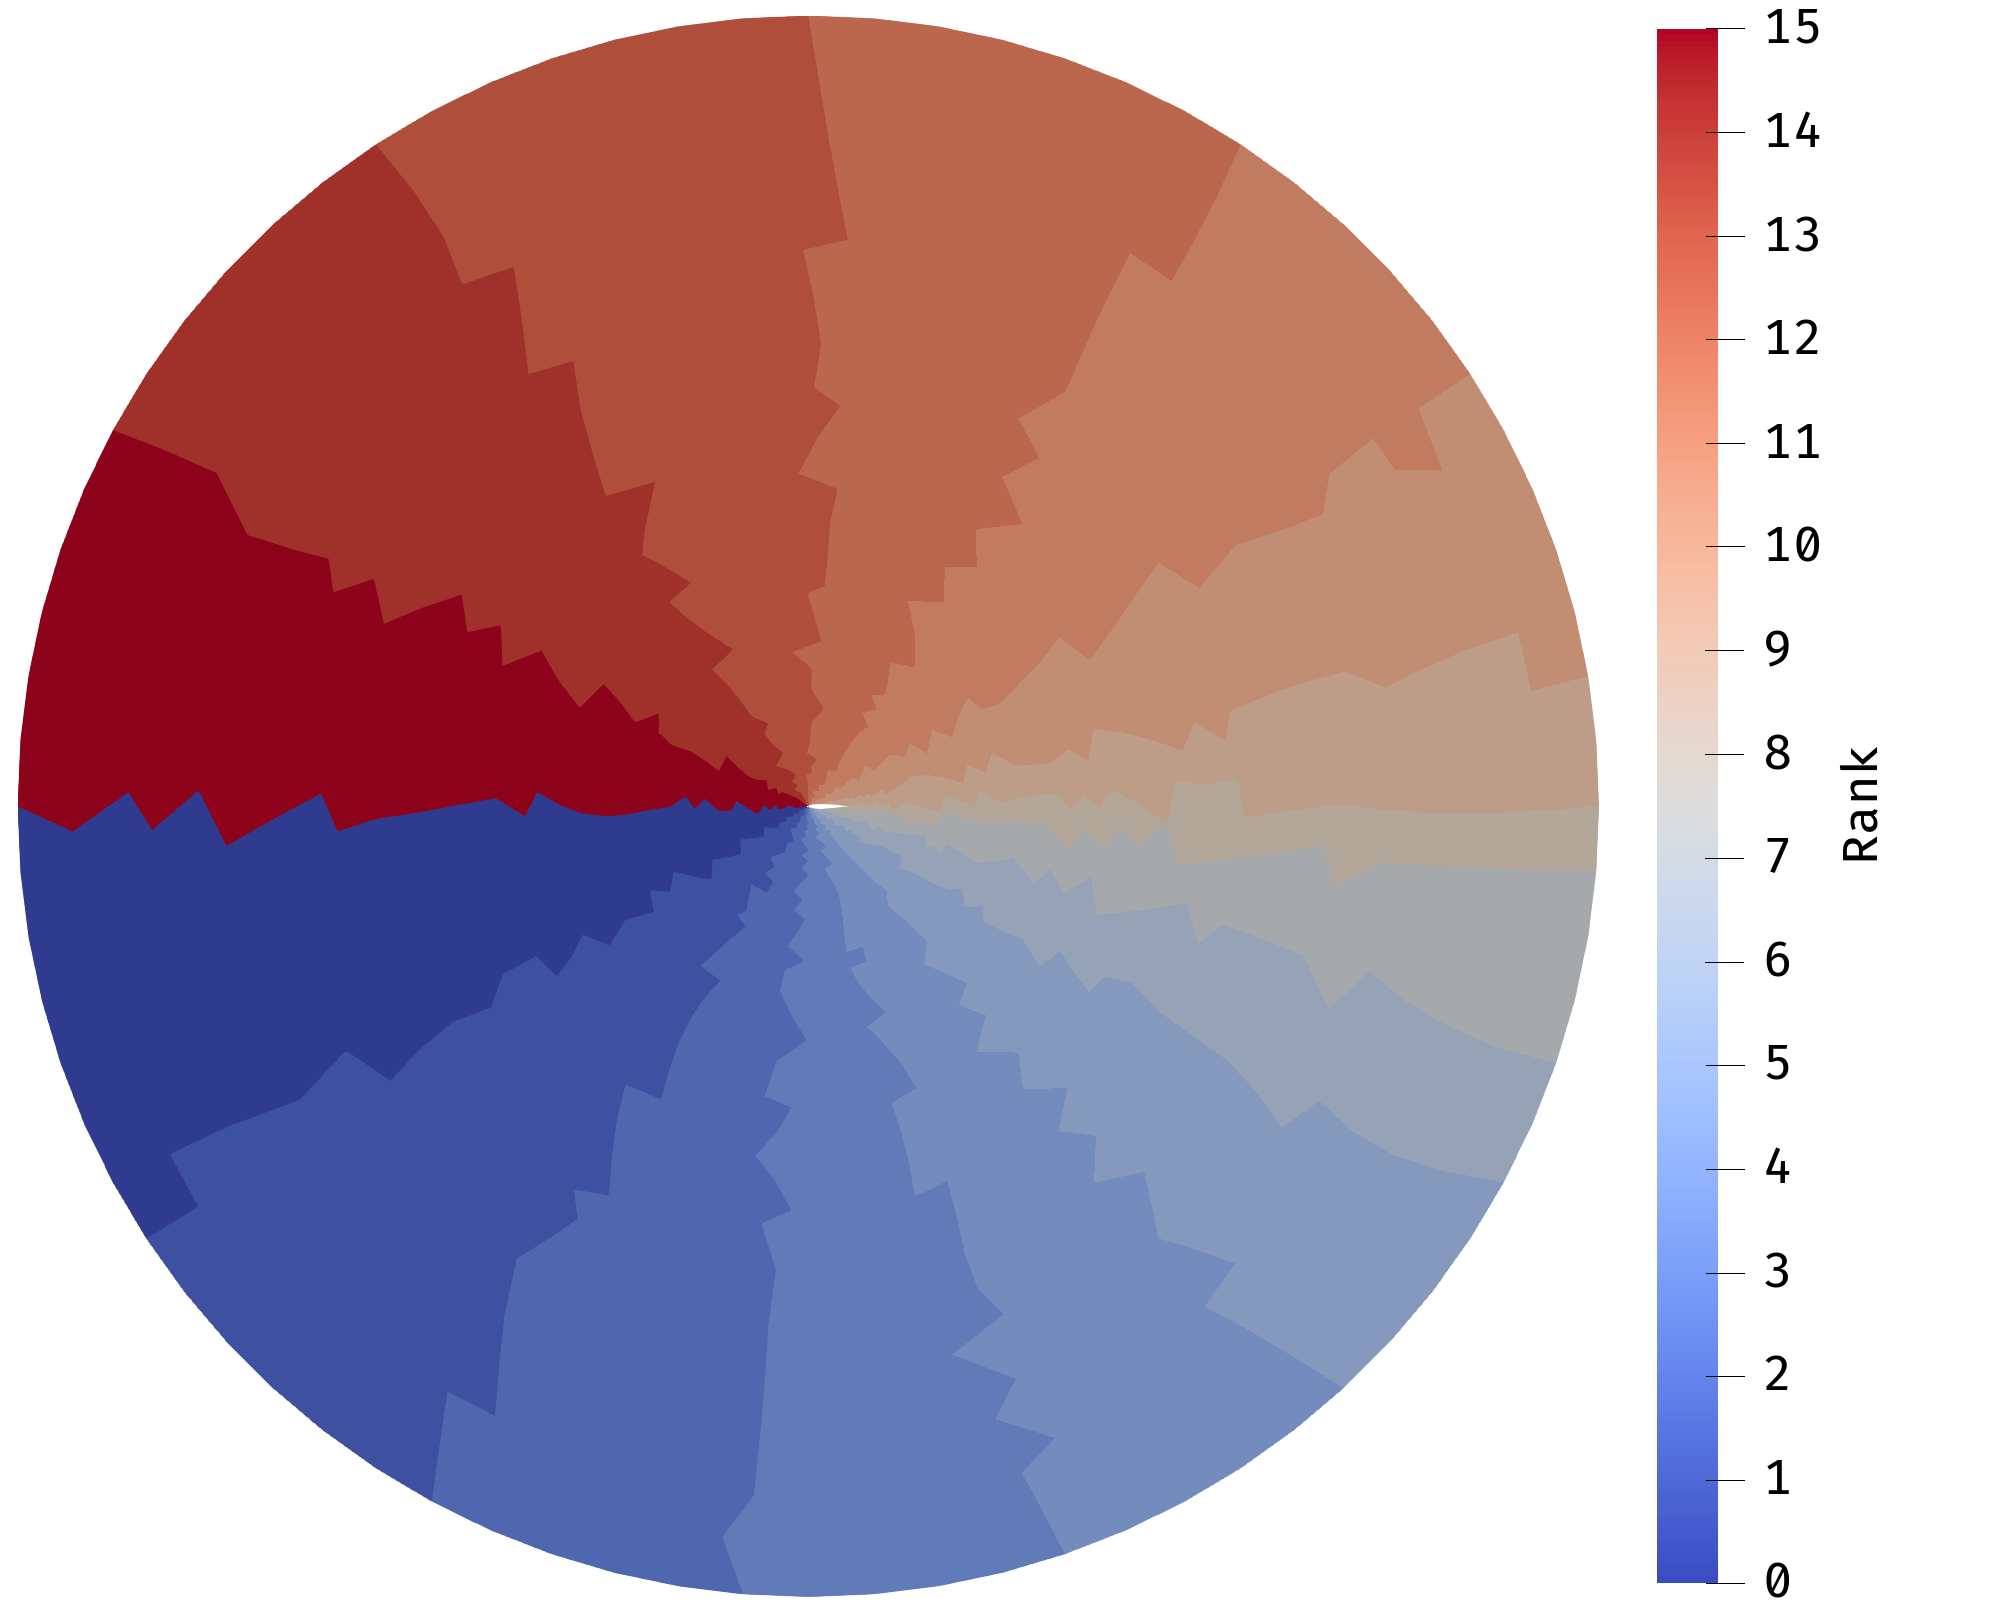
\includegraphics[width=0.45\textwidth]{Chapter_renumbering/media/rank_circular}\label{fig:rank_circular}}
	\caption{Circular sorted mesh: The elements are sorted according to their angle and the mesh is partitioned into \(16\) mesh blocks. (a) Ordering of the elements within the mesh (b) Mesh blocks once partitioned}\label{fig:mesh_circular}
\end{figure}

% doesn't work as well fof non-circles, good grouping but as there are more blocks they become thin
% slices with large boundaries. Then check next figure for how is locality, how elements are close
% their neighbours and numbered within blocks

\begin{figure}[H]
	\centering
	\includesvg[width=0.45\textwidth]{Chapter_renumbering/media/mesh_P0_before_adaptivity1_circular}
	\caption{Circular sorted mesh element ordering: The elements are very far from their neighbours.}\label{fig:mesh_circular_ordering}
\end{figure}

% is no good

% Figure about how we do it, that the curve is not defined but we map too square, make hilbert curve
% and sort elements according to into which index they fall. If multiple are in the same they keep
% their relative order. This is why we make very fine Hilbert curve

% figure about how we do it

% This is the ordering and blocks it gives

\begin{figure}[H]
	\centering
	\subfloat[Ordering]
	{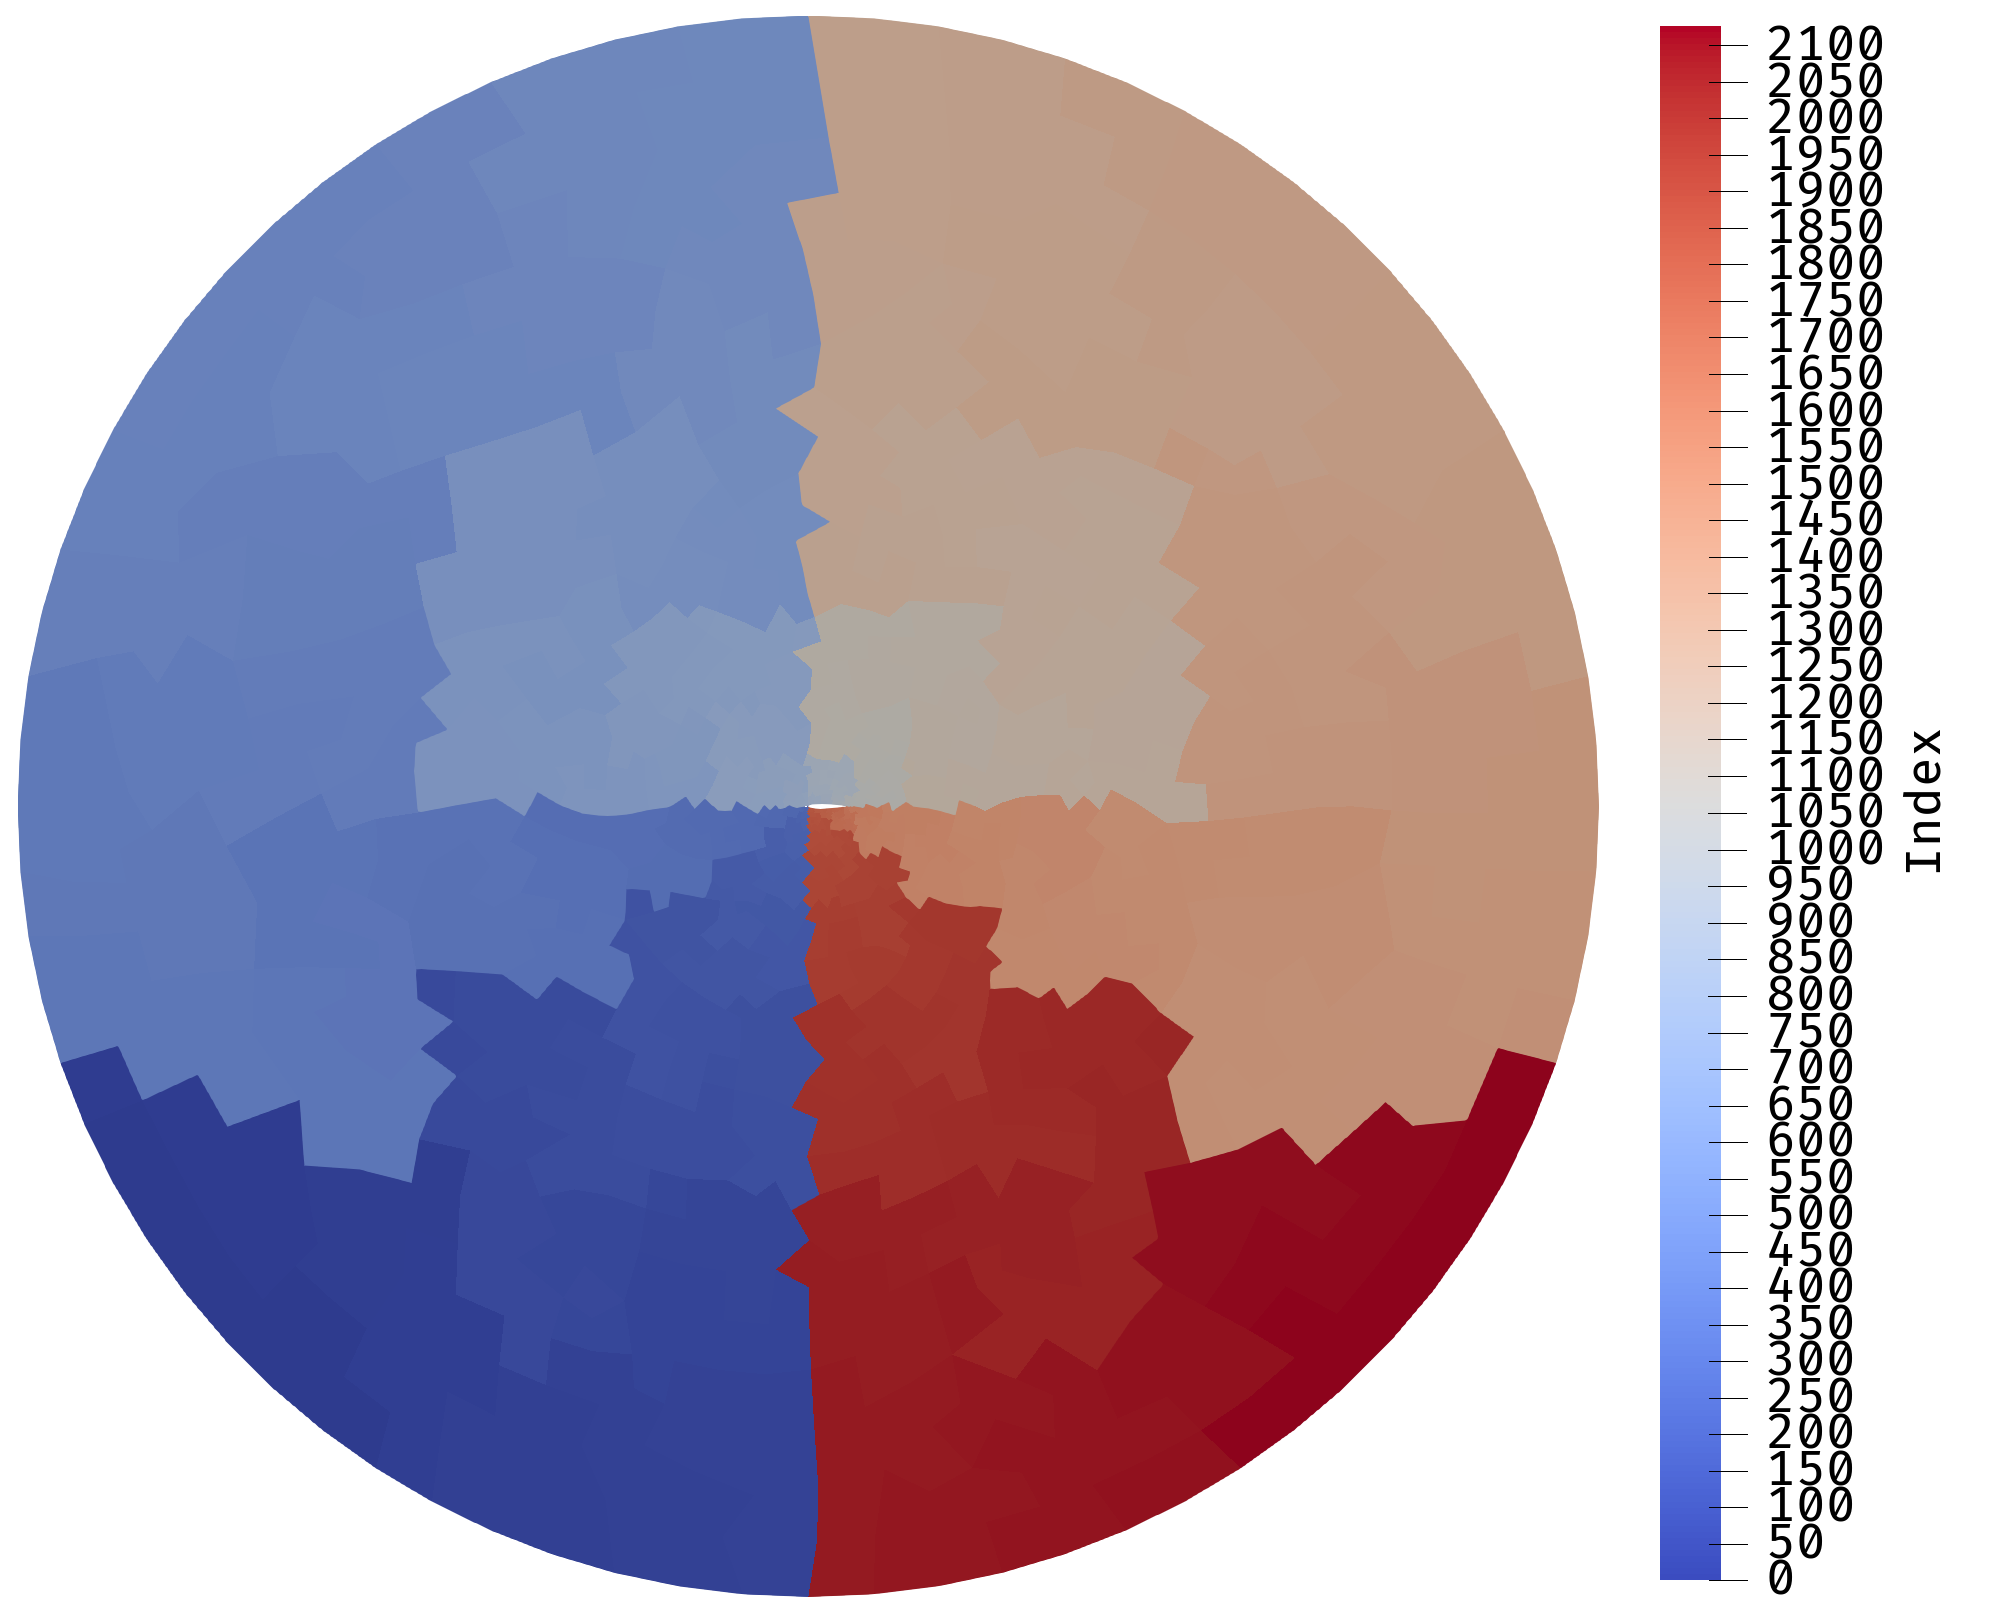
\includegraphics[width=0.45\textwidth]{Chapter_renumbering/media/ordering_hilbert}\label{fig:ordering_hilbert}}
	\subfloat[Rank]
	{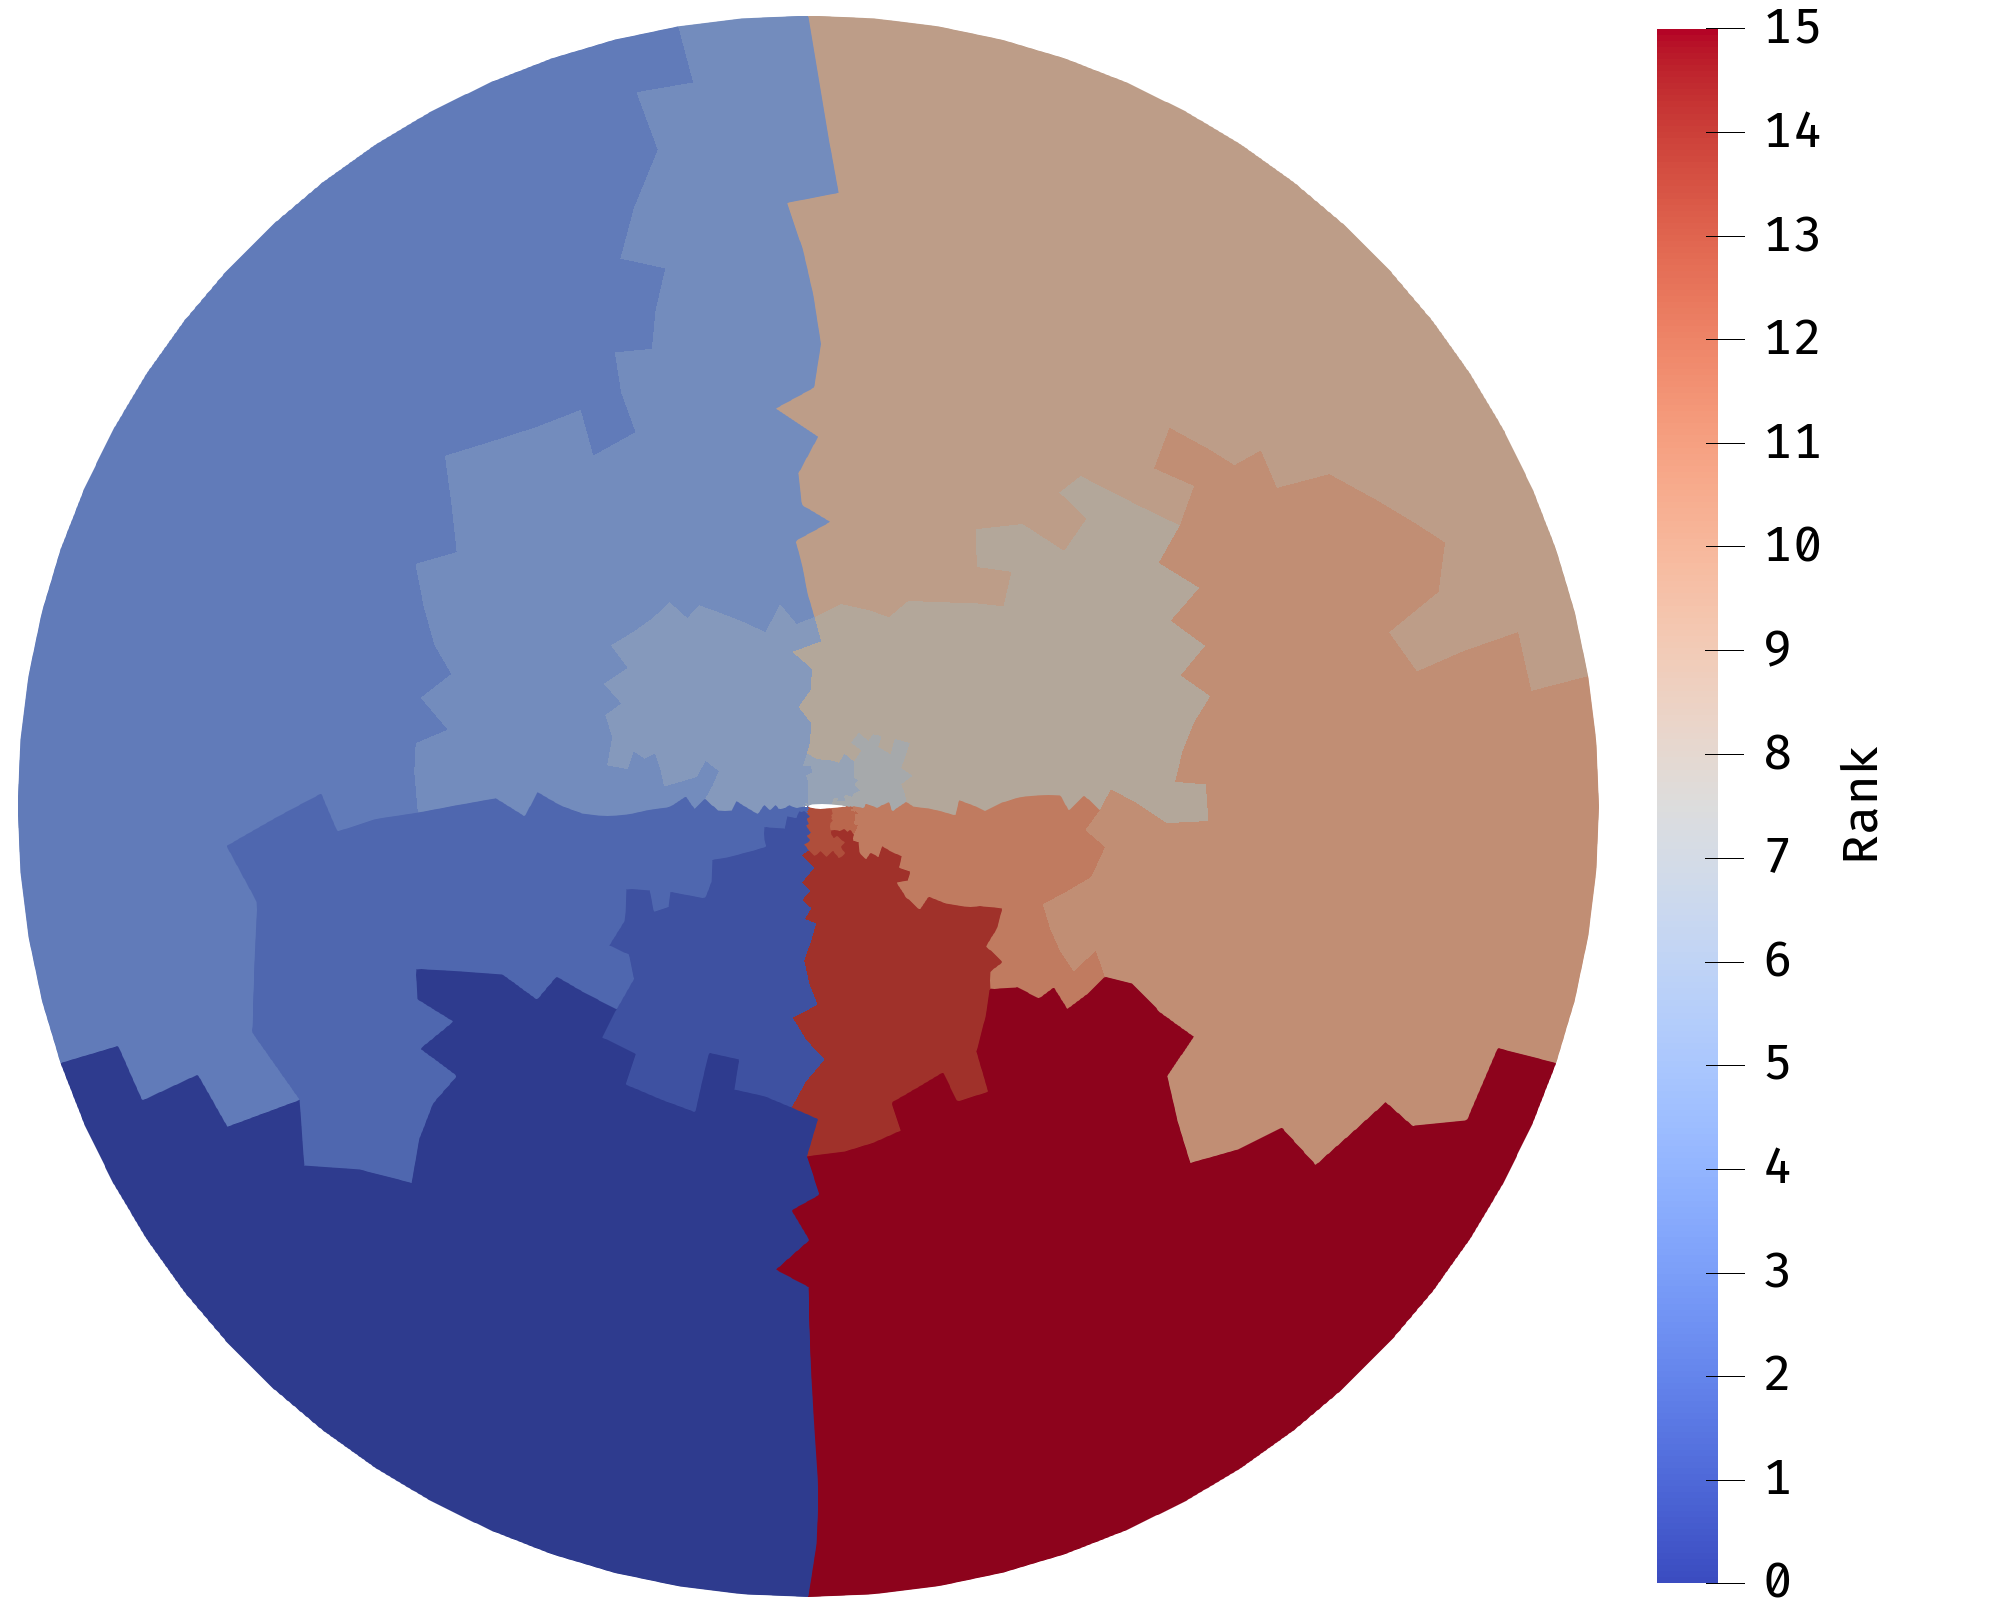
\includegraphics[width=0.45\textwidth]{Chapter_renumbering/media/rank_hilbert}\label{fig:rank_hilbert}}
	\caption{Pseudo-Hilbert sorted mesh:The elements are sorted according to their index along a Hilbert curve, and the mesh is partitioned into \(16\) mesh blocks. (a) Ordering of the elements within the mesh (b) Mesh blocks once partitioned}\label{fig:mesh_hilbert}
\end{figure}

% Good, good grouping elements and looks a bit like the real curve from ref{}
% Then we show the next figures, how is the ordering and how it works for refinement

\begin{figure}[H]
	\centering
	\subfloat[Before refinement]
	{\includesvg[width=0.45\textwidth]{Chapter_renumbering/media/mesh_P0_before_adaptivity1}\label{fig:mesh_P0_before_adaptivity1_far}}
	\subfloat[After refinement]
	{\includesvg[width=0.45\textwidth]{Chapter_renumbering/media/mesh_P0_after_adaptivity1}\label{fig:mesh_P0_after_adaptivity1_far}}
	\caption{\Acrlong{acr:AMR} with an unstructured mesh: The mesh is refined, created elements follow the initial pseudo-Hilbert curve. (a) Initial mesh (b) Mesh after a single refinement step}\label{fig:mesh_P0_adaptivity_far}
\end{figure}

\begin{figure}[H]
	\centering
	\subfloat[Solution time]
	{\includesvg[width=0.45\textwidth]{Chapter_renumbering/media/mesh_P0_before_adaptivity1_near}\label{fig:mesh_P0_before_adaptivity1_near}}
	\subfloat[Maximum error]
	{\includesvg[width=0.45\textwidth]{Chapter_renumbering/media/mesh_P0_after_adaptivity1_near}\label{fig:mesh_P0_after_adaptivity1_near}}
	\caption{\Acrlong{acr:AMR} with an unstructured mesh (detail): The mesh is refined, created elements follow the initial pseudo-Hilbert curve. There are jumps along the curve around the fuselage. (a) Initial mesh (b) Mesh after a single refinement step}\label{fig:mesh_P0_adaptivity_near}
\end{figure}

% Very good, refinement keeps the order of the curve well
% The order of the curve is good, but there are discontinuities near airfoil and weird jumps.
% Discontinuities: curve is not defined to have holes. Not too bad in this case since hole in middle
% Weird jumps:
% When too fine, the curve will "miss" elements by a little, giving surprising results. Future work:
% do with coarse grid, and refine for elements that fall in the same index only until they do not.